\section{Graphen}



%Abstract FEHLT

\subsection{Begriffe}

Als erstes m"ochten wir uns mit Graphen auseinander setzen. 
Wie wir oben gesehen haben kann man zum Beispiel das Liniennetz eines "OV-Betreibers als Graph darstellen. 


Im Allgemeinen ist ein Graph eine Struktur, die eine Menge von Objekten (z.B. Stationen) zusammen mit den zwischen diesen Objekten bestehenden Verbindungen (z.B. S-Bahn, Bus) repräsentiert. 

Die Objekte werden dabei \textbf{Knoten} des Graphen genannt. 
Die paarweisen Verbindungen zwischen Knoten heissen \textbf{Kanten}. 
Die Kanten können \textbf{gerichtet} oder \textbf{ungerichtet} sein, wenn die Verbindungen zwischen den Knoten eine Richtung beinhalten (oder nicht).
Dies wäre in unserem Fall eine Verbindung zwischen zwei Stationen, die nur in eine Richtung befahrbar ist; eine Einbahnstrasse.

Am einfachsten kann man Graphen zeichen, indem man Knoten durch Punkte und die Kanten durch Linien (ungerichtet) oder durch Pfeile im gerichteten Fall darstellt. 

\begin{mbsp}
%\paragraph{Beispiel:}
Anschauliche Beispiele für Graphen sind ein Stammbaum oder das S-Bahn-Netz (s. Abb.~\ref{fig:sbahn}) einer Stadt. 
Bei einem Stammbaum stellt jeder Knoten ein Familienmitglied dar und jede Kante ist eine Verbindung zwischen einem Elternteil und einem Kind. 
In einem S-Bahn-Netz stellt jeder Knoten eine S-Bahn-Station dar und jede Kante eine direkte Zugverbindung zwischen zwei Stationen.
\end{mbsp}
%\begin{figure}[htb]
%\begin{center}
%
%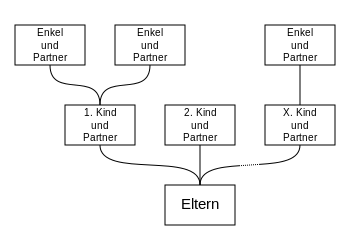
\includegraphics[width=.67\textwidth]{../fig/stammbaum.png}
%%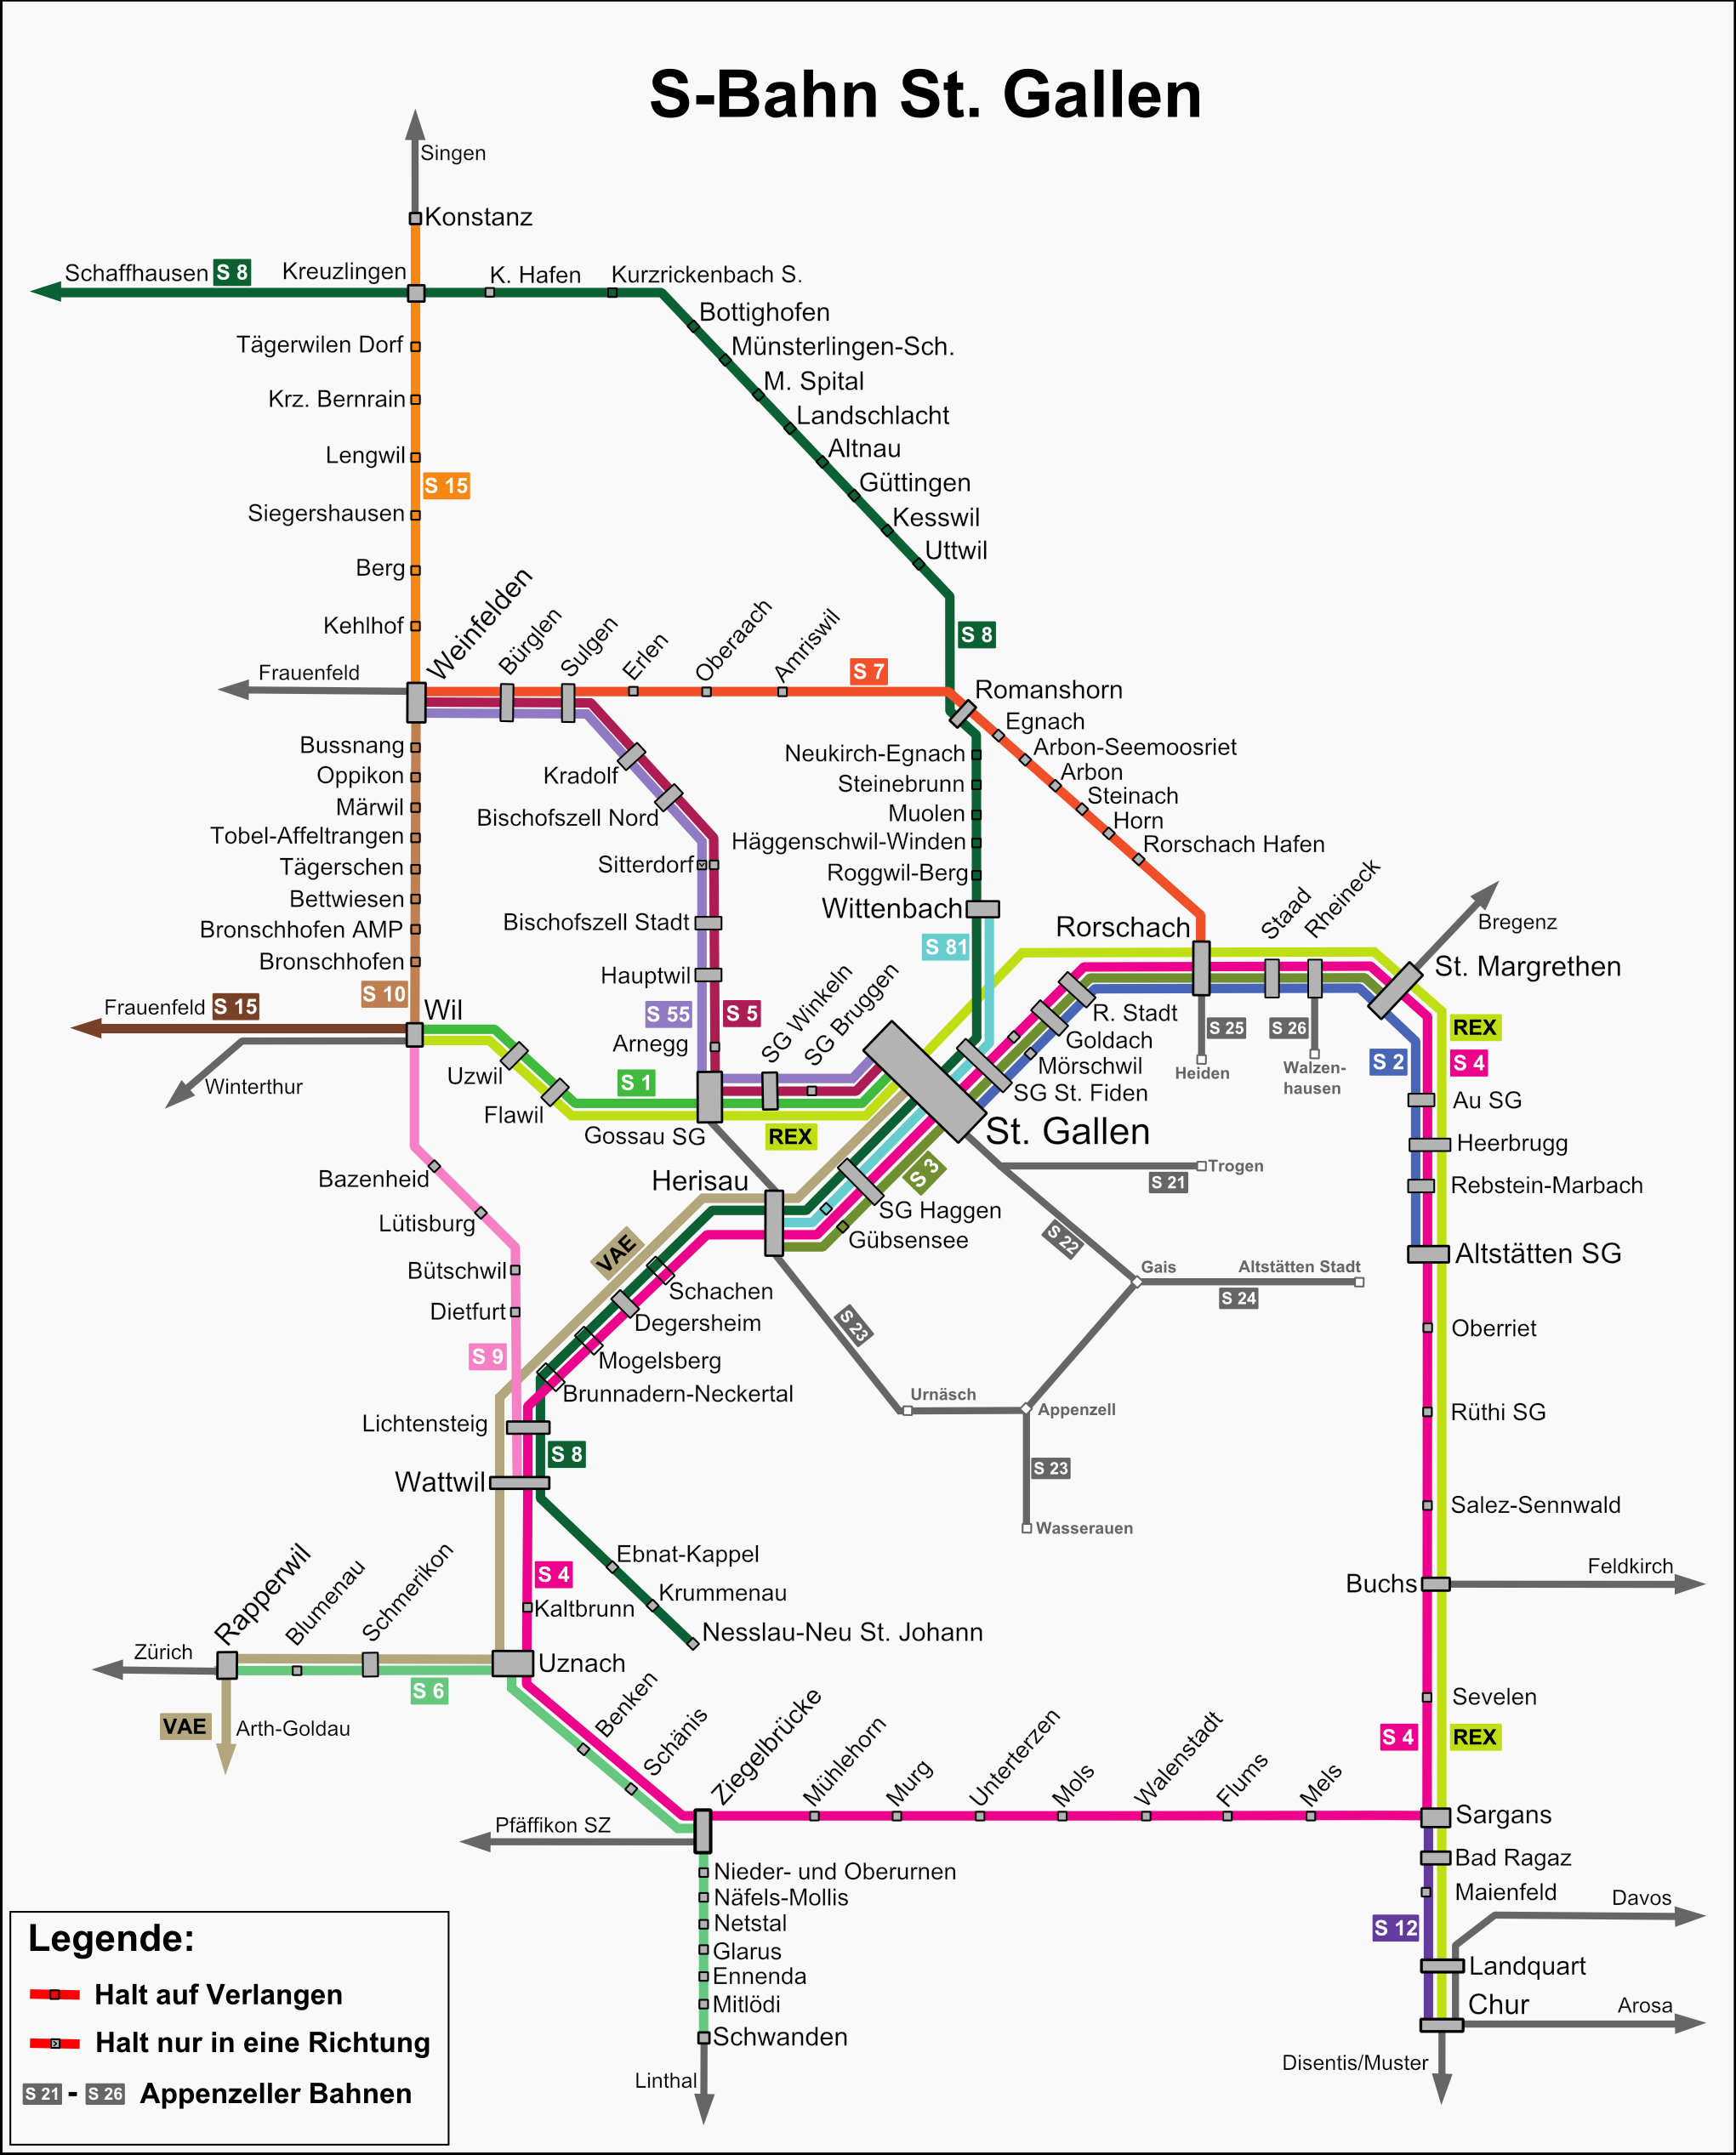
\includegraphics[width=.45\textwidth]{../fig/sbahn_netz.png}
%\caption{Darstellung eines Stammbaumes als (ungerichteter) Graph.
%Jedes Familienmitglied (Enkel, Kind, Eltern) ist ein Knoten und die Kanten bilden die Verbindungen zwischen Eltern und Kindern.
%%https://upload.wikimedia.org/wikipedia/commons/thumb/c/c1/Stammbaum.svg/400px-Stammbaum.svg.png
%}
%\label{fig:stammbaum}
%
%\end{center}
%\end{figure}

\begin{figure}[htb]
\begin{center}

%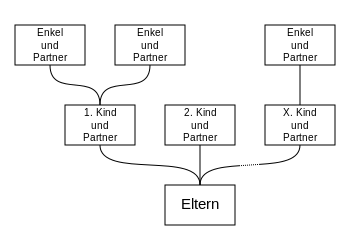
\includegraphics[width=.7\textwidth]{../fig/stammbaum.png}
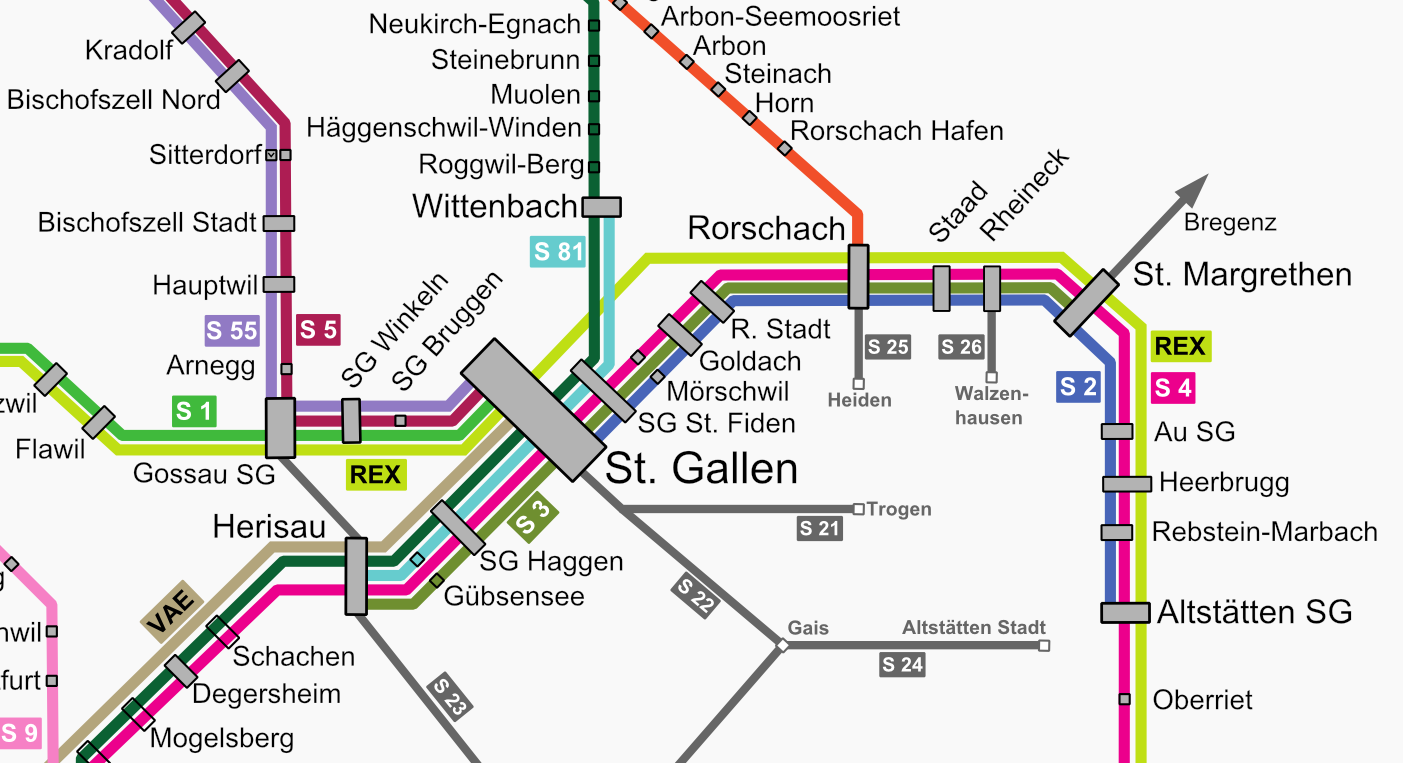
\includegraphics[width=.67\textwidth]{../fig/sbahn_netz_ausschnitt.png}
\caption{Darstellung eines Ausschnitts des Sankt Galler S-Bahn-Netzes als (ungerichteter) Graph.
Jede Station bildet dabei einen Knoten und die Verbindung zwischen den Knoten ist eine Kante.
%https://upload.wikimedia.org/wikipedia/commons/1/19/Map_S-Bahn_St._Gallen_%28schematic%29.png
}

\label{fig:sbahn}
\end{center}
\end{figure}


\subsection{Definitionen}

Wir führen direkt die Definition für Graphen ein wobei wir zwei Arten unterscheiden: gerichtete und ungerichtete Graphen.

\begin{mdef}
%\paragraph{Graph:}
Mathematisch besteht ein \textbf{Graph} $G=(V,E)$ aus einer \textbf{Menge} von \textbf{Knoten} $V$ (engl. \emph{vertex}) und einer \textbf{Menge} von \textbf{Kanten} $E$ (engl. \emph{edge}).
Die Anzahl Knoten wird mit $|V|$ und die Anzahl Kanten mit $|E|$ bezeichnet.
\end{mdef}



\begin{mdef}
%\paragraph{Ungerichteter Graph:}
Jede Kante eines \textbf{ungerichteten Graphen} $e$ besteht aus zwei Knoten $v_1$ und $v_2$ und wird selbst als Menge dargestellt: $e= \{v_1,v_2\}$.
Die Reihenfolge spielt dabei keine Rolle: $\{v_1,v_2\} = \{v_2,v_1\}$.
\end{mdef}


\begin{mbsp}
%\paragraph{Beispiele:}
Die Abblidung~\ref{fig:bsp:ugraph} zeigt einen ungerichteten Graphen mit 5 Knoten und 7 ungerichteten Kanten.
\end{mbsp}

\begin{figure}[htb]
\begin{center}
\begin{tikzpicture}[-,>=stealth',shorten >=1pt,auto,node distance=2.8cm,
                    semithick, style=circle]
  \tikzstyle{wstate}=[fill=white,text=black,draw=black]
%  \tikzstyle{gstate}=[fill=gray,text=black,draw=black]
%  \tikzstyle{bstate}=[fill=black,text=white,draw=black]
  

  \node[wstate]         (1) 			 {$1$};
    \node[wstate] 		(0) [below of=1] {$0$};
  \node[wstate]         (2) [right of=1] {$2$};
  \node[wstate]         (3) [below right of=2] {$3$};
  \node[wstate]         (4) [below of=2]       {$4$};
%  \node[wstate]         (2) [above right of=4]       {$2$};

  \path (0) edge              node {} (1)
            edge              node {} (2)
            edge              node {} (4)
        (1) edge 			  node {} (2)
        (3) edge              node {} (2)
	        edge  			  node {} (4)
        (2) edge 			  node {} (4);
%            edge              node {} (4)
%        (4) edge [bend left]  node {} (0);
\end{tikzpicture}
\caption{Ein gerichteter Graph mit 6 Knoten.
}
\label{fig:bsp:ugraph}
\end{center}
\end{figure}

Die mathematische Darstellung des Graphen lautet:

\[\quad G = (V, E); \quad V = \{0,1,2,3,4\}; \] 
\[\quad E =  \{ \{1,2\},\{1,0\},\{2,0\},\{2,4\},\{2,3\}, \{3,4\}, \{4,0\}. \}  \]

\begin{mdef}
%\paragraph{Gerichteter Graph:}
Jede Kante eines \textbf{gerichteten Graphen} $e$ besteht aus einem Startknoten $v_1$ und einem Zielknoten $v_2$ und wird selbst als 2-Tupel dargestellt: $e= (v_1,v_2)$. 
Hierbei spielt die Reihenfolge ein Rolle: $(v_1,v_2) \neq (v_2,v_1)$. 
\end{mdef}


\begin{mbsp}
%\paragraph{Beispiele:}
Die Abblidung~\ref{fig:bsp:ggraph} zeigt einen gerichteten Graphen mit 6 Knoten und 7 Kanten. 
\end{mbsp}

\begin{figure}[htb]
\begin{center}
\begin{tikzpicture}[->,>=stealth',shorten >=1pt,auto,node distance=2.8cm,
                    semithick, style=circle]
  \tikzstyle{wstate}=[fill=white,text=black,draw=black]
%  \tikzstyle{gstate}=[fill=gray,text=black,draw=black]
%  \tikzstyle{bstate}=[fill=black,text=white,draw=black]
  

  \node[wstate]         (1) 			 		{$1$};
  \node[wstate]         (2) [right of=1]		{$2$};
  \node[wstate]         (3) [right of=2]		{$3$};
  \node[wstate]         (4) [below of=1]		{$4$};
  \node[wstate]         (5) [right of=4]		{$5$};
  \node[wstate] 		(0) [right of=5]		{$0$};

%  \path (0) edge	[loop right]	node {} (0)
  \path (1) edge 					node {} (2)
        	edge 					node {} (4)
        (2) edge            		node {} (5)
        (3) edge 					node {} (5)
        	edge					node {} (0)
        (4) edge   					node {} (2)
        (5) edge   					node {} (4);
        %[bend left]
\end{tikzpicture}

\caption{Ein gerichteter Graph mit 6 Knoten.
}
\label{fig:bsp:ggraph}
\end{center}
\end{figure}



%\begin{figure}[htb]
%\begin{center}
%
%%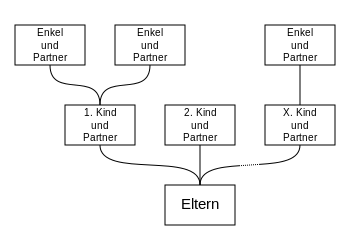
\includegraphics[width=.7\textwidth]{../fig/stammbaum.png}
%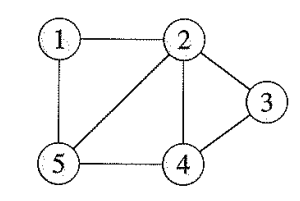
\includegraphics[width=.45\textwidth]{../fig/graph_ug_01.png}\hfill
%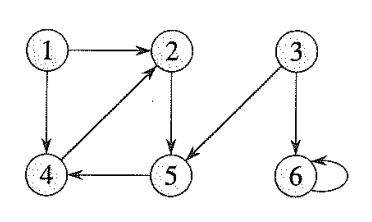
\includegraphics[width=.45\textwidth]{../fig/graph_ge_01.png}
%\caption{\emph{Links:} Ein ungerichteter Graph mit 5 Knoten. 
%\emph{Rechts:} Ein gerichteter Graph mit 6 Knoten.
%}
%\label{fig:bsp:ugraph}
%\end{center}
%\end{figure}

Die mathematische Darstellung des Graphen lautet:

\[\quad G = (V, E); \quad V = \{0,1,2,3,4,5\}; \] 
\[\quad E =  \{ (1,2),(1,4), (2,5), (3,5), (3,0), (4,2), (5,4)\}.  \]

\begin{aufg}
%\paragraph{Aufgabe:}
Bilden Sie für folgenden Graph (Abb.~\ref{fig:auf:graph}) die entsprechende mathematische Darstellung $G=(V,E)$.
\end{aufg}


\begin{figure}[htb]
\begin{center}
\begin{tikzpicture}[->,>=stealth',shorten >=1pt,auto,node distance=2.8cm,
                    semithick, style=circle]
  \tikzstyle{wstate}=[fill=white,text=black,draw=black]
%  \tikzstyle{gstate}=[fill=gray,text=black,draw=black]
%  \tikzstyle{bstate}=[fill=black,text=white,draw=black]
  
  \node[wstate] 		(0)                    {$0$};
  \node[wstate]         (1) [above of=0] {$1$};
  \node[wstate]         (2) [right of=1] {$2$};
  \node[wstate]         (3) [below right of=2] {$3$};
  \node[wstate]         (4) [below of=2]       {$4$};

  \path (0) edge              node {} (1)
            edge              node {} (2)
%        (1) edge [loop above] node {} (1)
        (1)  edge              node {} (2)
        (3) edge              node {} (1)
            edge [bend left]  node {} (4)
%        (2) edge [loop below] node {} (2)
        (2) edge              node {} (0)
        (4) edge [bend left]  node {} (0);
\end{tikzpicture}
\caption{Ein gerichteter Graph.}
\label{fig:auf:graph}
\end{center}
\end{figure}


\begin{aufg}
%\paragraph{Aufgabe:} 
Zeichnen Sie den entsprechenden Graph, der zu folgender Mathematischen Darstellung gehört:

\[ \quad G = (V, E); \quad V = \{0,1,2,3,4,5,6\}; \] 
\[\quad E =  \{ (1,3),(1,6), (2,1), (3,4), (4,2), (5,4), (6,3)\}. \]

\end{aufg}


\begin{mdef}
%\paragraph{Adjazenzmatrix:}
Für einen Graphen $G=(V,E)$ nehmen wir an, dass die Knoten in beliebiger Weise von 0 bis $|V|-1$ nummeriert sind.
So bildet die \textbf{Adjazenzmatrix-Darstellung} des Graphen $G$ eine $|V| \times |V|$-Matrix $A=a_{ij}$ mit den Elementen

\[ a_{ij} = 
  \begin{cases}
    1   & \quad \text{falls } (i,j) \in E, \\
   0   & \quad \text{sonst}
  \end{cases}.
\]

Für ungerichtete Graphen ersetzt man $(i,j) \text{ durch } \{i,j\}$.
\end{mdef}

Das Element $a_{ij}$ hat zwei Indizes $i$ und $j$. Der erste Index ($i$) gibt uns die Zeile der Matrix an und der zweite ($j$) die Spalte:

\[
A = \begin{pmatrix}
  a_{00} & a_{01} & a_{02} & \cdots \\
  a_{10} & a_{11} & a_{12} & \cdots \\
  a_{20} & a_{21} & a_{22} & \cdots \\
  \vdots & \vdots & \vdots & \ddots \\
\end{pmatrix}
\]

Man muss bei ungerichteten Graphen beachten, dass eine Verbindung zwischen zwei Knoten in beide Richtungen durchlaufen werden kann und beide Verbindungen in die Matrix eingetragen werden müssen. 

\begin{mbsp}
%\paragraph{Beispiele:}
Die Adjazenz-Matrizen $A$ zu dem Graph in Abb.~\ref{fig:bsp:ugraph} lautet:

\[ A =  \begin{pmatrix}
  0 & 1 & 1 & 0 & 1 \\
  1 & 0 & 1 & 0 & 0 \\
  1 & 1 & 0 & 1 & 1  \\
  0 & 0 & 1 & 0 & 1 \\
  1 & 0 & 1 & 1 & 0 \\
 \end{pmatrix}
\]
\end{mbsp}


\begin{mbsp}
%\paragraph{Beispiele:}
Die Adjazenz-Matrizen $A$ zu dem Graph in Abb.~\ref{fig:bsp:ggraph} lautet:

\[ 
A =  \begin{pmatrix}
  0 & 0 & 0 & 0 & 0 & 0 \\
  0 & 0 & 1 & 0 & 1 & 0 \\
  0 & 0 & 0 & 0 & 0 & 1 \\
  1 & 0 & 0 & 0 & 0 & 1 \\
  0 & 0 & 1 & 0 & 0 & 0 \\
  0 & 0 & 0 & 0 & 1 & 0 \\
 \end{pmatrix}
  \]
\end{mbsp}

\begin{aufg}
%\paragraph{Aufgabe:} 
Bilden Sie für den Graphen aus Abbildung~\ref{fig:auf:graph} die entsprechende Adjazenzmatrix $G=(V,E)$.
\end{aufg}



\begin{aufg}
%\paragraph{Aufgabe:} 
Zeichnen Sie zu folgender Adjazenzmatrix den entsprechenden Graphen.
Überlegen Sie sich zu erst, ob es sich um einen gerichteten oder ungerichteten Graphen handelt.


\[A =  \begin{pmatrix}
  0 & 1 & 0 & 0 & 1 & 0 \\
  0 & 0 & 1 & 0 & 1 & 0 \\
  0 & 1 & 0 & 0 & 1 & 1 \\
  1 & 0 & 0 & 0 & 0 & 0 \\
  0 & 1 & 0 & 1 & 0 & 0 \\
  0 & 0 & 1 & 0 & 1 & 0 \\
 \end{pmatrix}
  \]
  
\end{aufg}

\paragraph{Programmierung:}
Damit auch ein Computerprogramm einen Graphen lesen kann, kann man diesen als Liste von Listen darstellen. 
Der folgende Befehl erstellt eine Liste mit drei einträgen.
\begin{lstlisting}[language=Python,basicstyle=\small,tabsize=3]
a = [1,5,3]
print a[1]
\end{lstlisting}
Mit dem zweiten Befehl wird das zweite Element ausgegeben - in diesem Fall 5. 
Es ist wichtig zu beachten, dass in Python das erste Element mit 0 markiert ist. 
Damit wir eine Matrix speichern speichern wir nun mehrere Listen in einer Liste
\begin{lstlisting}[language=Python,basicstyle=\small,tabsize=3]
A = [ [0,3,5], [2,4,1], [-1,7,9] ]
print A[1]
print A[0][2]
\end{lstlisting}
Die Ausgabe ergibt:
\begin{lstlisting}[language=Python,basicstyle=\small,tabsize=3]
[2,4,1]
5
\end{lstlisting}
Wir speichern also Zeile für Zeile eine Matrix in diesem Beispiel wurde folgende Matrix gespeichert:

\[A =  \begin{pmatrix}
 0 & 3 & 5 \\
 2 & 4 & 1 \\
 -1& 7 & 9 \\
 \end{pmatrix}
  \]


\begin{aufg}
Stellen Sie folgende Matrix in Python dar. Überprüfen Sie dabei ihre Eingabe indem Sie die zweite Zeile und das Element $a_{23}$ ausgeben (print). 

\[ A =  \begin{pmatrix}
  0 & 1 & 0 & 0 & 1 \\
  1 & 0 & 1 & 0 & 0 \\
  1 & 1 & 0 & 1 & 1  \\
  0 & 0 & 1 & 0 & 1 \\
  1 & 0 & 1 & 1 & 0 \\
 \end{pmatrix}
\]

\end{aufg}

%\begin{aufg}
%%\paragraph{Programmierung:}
%Damit man einen Graphen in einer Textdatei speichern und lesen kann, benutzt man häufig ';' (Semicolon) um die Zahlen einer Zeile zu trennen. 
%Mit einem Absatz wird eine neue Zeile der Matrix bestimmt. 
%Schreiben Sie ein Programm \textsc{NicePrint($graph$)}, das die Adjazenzliste eines Graphen auf den Bildschirm ausgibt.
%%Benutzen Sie dafür das vorgegebene Programm, welches Graphen aus einer Textdatei einlesen kann und überprüfen Sie die Ausgabe mit den Textdateien.
%\end{aufg}


\begin{mdef}
%\paragraph{Nachbarn:} 
Zwei Knoten sind zueinander \textbf{benachbart}, wenn eine direkte Verbindung durch eine Kante besteht. 
In einem ungerichteten Graphen sind immer beide Knoten benachbart. 
Hingegen spielt in einem gerichteten Graphen die Richtung der Kante eine Rolle, so dass die Nachbarschaft nur in die Richtung gelten kann, in welche der Pfeil zeigt.

\end{mdef}

\begin{mbsp}
In ungerichteten Graphen sind immer die zwei Knoten benachbart, wenn sie verbunden sind. 
So ist in der folgenden Abbildung~\ref{fig:bsp:unbar} auf der rechten Seite der Knoten 2 und 3 benachbart. 
\begin{figure}[htb]
\begin{center}
\begin{tikzpicture}[-,>=stealth',shorten >=1pt,auto,node distance=2.8cm,
                    semithick, style=circle]
  \tikzstyle{wstate}=[fill=white,text=black,draw=black]
   \node[wstate]         (2) [right of=1] {$2$};
  \node[wstate]         (3) [right of=2] {$3$};
%  \node[wstate]         (4) [below of=2]       {$4$};

  \path (2) edge              node {} (3);
\end{tikzpicture}

\caption{Zwei Knoten in einem ungerichteten Graphen.}
\label{fig:bsp:unbar}
\end{center}
\end{figure}
Bei gerichteten Graphen jedoch spielt die Richtung eine Rolle. So hat im folgenden Beispiel (Abb.~\ref{fig:bsp:gnbar}) der Knoten 0 den Nachbarknoten 1, aber der Knoten 1 hat keinen Nachbarknoten. 
\begin{figure}[htb]
\begin{center}
\begin{tikzpicture}[->,>=stealth',shorten >=1pt,auto,node distance=2.8cm,
                    semithick, style=circle]
  \tikzstyle{wstate}=[fill=white,text=black,draw=black]
%  \tikzstyle{gstate}=[fill=gray,text=black,draw=black]
%  \tikzstyle{bstate}=[fill=black,text=white,draw=black]
  
  \node[wstate] 		(0)                    {$0$};
  \node[wstate]         (1) [right of=0] {$1$};
%  \node[wstate]         (2) [right of=1] {$2$};
%  \node[wstate]         (3) [right of=2] {$3$};
%  \node[wstate]         (4) [below of=2]       {$4$};

  \path (0) edge              node {} (1);
\end{tikzpicture}
\caption{Zwei gerichteten Graphen.}
\label{fig:bsp:gnbar}
\end{center}
\end{figure}
\end{mbsp}


Man kann die Nachbarn direkt aus der Adjazenzmatrix ablesen. 
Dazu betrachtet man die Zeile des Knoten und immer wenn eine Eins geschrieben steht, heisst dass, der Knoten in der entsprechenden Spalte ein Nachbar ist.

\begin{mbsp}
%\paragraph{Beispiel:}
Betrachten wir nochmal den Graphen der Abbildung~\ref{fig:bsp:ggraph} mit seiner Adjazenzmatrix:


\begin{figure}[htb]
\begin{center}
\begin{tikzpicture}[->,>=stealth',shorten >=1pt,auto,node distance=2.8cm,
                    semithick, style=circle]
  \tikzstyle{wstate}=[fill=white,text=black,draw=black]
%  \tikzstyle{gstate}=[fill=gray,text=black,draw=black]
%  \tikzstyle{bstate}=[fill=black,text=white,draw=black]
  

  \node[wstate]         (1) 			 		{$1$};
  \node[wstate]         (2) [right of=1]		{$2$};
  \node[wstate]         (3) [right of=2]		{$3$};
  \node[wstate]         (4) [below of=1]		{$4$};
  \node[wstate]         (5) [right of=4]		{$5$};
  \node[wstate] 		(0) [right of=5]		{$0$};

%  \path (0) edge	[loop right]	node {} (0)
  \path (1) edge 					node {} (2)
        	edge 					node {} (4)
        (2) edge            		node {} (5)
        (3) edge 					node {} (5)
        	edge					node {} (0)
        (4) edge   					node {} (2)
        (5) edge   					node {} (4);
        %[bend left]
\end{tikzpicture}

\caption{Ein gerichteter Graph mit 6 Knoten.
}
\label{fig:bsp:ggraph2}
\end{center}
\end{figure}



\[ 
A =  \begin{pmatrix}
  1 & 0 & 0 & 0 & 0 & 0 \\
  \textbf{0} & \textbf{0} & \textbf{1} & \textbf{0} & \textbf{1} & \textbf{0} \\
  0 & 0 & 0 & 0 & 0 & 1 \\
  1 & 0 & 0 & 0 & 0 & 1 \\
  0 & 0 & 1 & 0 & 0 & 0 \\
  0 & 0 & 0 & 0 & 1 & 0 \\
 \end{pmatrix}
  \]
  
  
Hier hat der Knoten 1 die Nachbarn 2 und 4.
Die entsprechende Zeile ist \textbf{fett} markiert in der Matrix.
Umgekehrt hat der Knoten 2 nur den Knoten 5 als Nachbar und nicht den Knoten 1.
%Auch dies kann man wieder aus der zweiten Reihe der Adjazenzmatrix $A_r$ ablesen.
\end{mbsp}

\begin{aufg}
%\paragraph{Aufgabe:} 
Welche Nachbarn hat der Knoten 3, der Knoten 1 und der Knoten 0 des folgenden Graphen in Abbildung~\ref{fig:auf:graph2}.


\begin{figure}[htb]
\begin{center}
\begin{tikzpicture}[->,>=stealth',shorten >=1pt,auto,node distance=2.8cm,
                    semithick, style=circle]
  \tikzstyle{wstate}=[fill=white,text=black,draw=black]
%  \tikzstyle{gstate}=[fill=gray,text=black,draw=black]
%  \tikzstyle{bstate}=[fill=black,text=white,draw=black]
  
  \node[wstate] 		(0)                    {$0$};
  \node[wstate]         (1) [above of=0] {$1$};
  \node[wstate]         (2) [right of=1] {$2$};
  \node[wstate]         (3) [below right of=2] {$3$};
  \node[wstate]         (4) [below of=2]       {$4$};

  \path (0) edge              node {} (1)
            edge              node {} (2)
%        (1) edge [loop above] node {} (1)
        (1)    edge              node {} (2)
        (3) edge              node {} (1)
            edge [bend left]  node {} (4)
%        (2) edge [loop below] node {} (2)
        (2)    edge              node {} (0)
        (4) edge [bend left]  node {} (0);
\end{tikzpicture}
\caption{Ein gerichteter Graph.}
\label{fig:auf:graph2}
\end{center}
\end{figure}

\end{aufg}


\begin{aufg}
Bestimmen Sie die Nachbarknoten der Knoten 0,2 und 4 der folgenden Adjazenzmatrix. 
Gehen Sie dabei davon aus, dass wie immer die Knoten von Null an durchnummeriert sind.


\[ A =  \begin{pmatrix}
  0 & 1 & 0 & 0 & 1 \\
  1 & 0 & 1 & 0 & 0 \\
  1 & 1 & 0 & 1 & 1  \\
  0 & 0 & 1 & 0 & 1 \\
  1 & 0 & 1 & 1 & 0 \\
 \end{pmatrix}
\]

\end{aufg}



\begin{aufg}
%\paragraph{Programmierung:}
Implementieren Sie eine Funktion \textsc{Nachbarknoten($graph$, $knoten$)}: Sie hat als Input einen Graphen ($graph$) und einen Knoten ($knoten$) und gibt als Output eine Liste von Nachbarknoten des Knoten aus. Testen Sie die Funktion, indem Sie sie mit verschiedenen Knoten aus einem Graphen aufrufen.
\end{aufg}

\subsection{Zusammenfassung und Kontrollaufgaben}

In diesem Kapitel haben Sie die Darstellung von Graphen wiederholt. 
Insbesondere haben Sie verschiedene Darstellungen der Graphen kennen gelernt: Zeichnung, Menge von Kanten und Knoten und Adjazenzmatrix.
Zusätzlich kennen Sie den Unterschiede zwischen gerichteten und ungerichteten Graphen, welche sich auch in den verschiedenen Darstellungen zeigen. 
Sie können auch die Graphen in einem Programm mithilfe von Listen in Listen darstellen und ausgeben. 
Zusätzlich haben Sie das Konzept der benachbarten Knoten (Nachbar) in Graphen kennengelernt und können Nachbarknoten in verschiedenen Darstellungsformen bestimmen. 


%\subsection{Kontrollaufgaben}

%\begin{enumerate}
\begin{kontr}
Beschreiben Sie Unterschiede und Gemeinsamkeiten von gerichteten und ungerichteten Graphen.
\end{kontr}


\begin{kontr}
Nennen Sie drei weitere Beispiele aus dem Alltag für Graphen. 
Bestimmen Sie dabei immer was die Knoten und was die Kanten darstellen. 
Handelt es sich dabei um gerichtete oder ungerichtete Graphen?
\end{kontr}


\begin{kontr}
Betrachten Sie folgenden Graphen (s. Abb.~\ref{fig:kont:graph}) und bestimmen Sie seine Knoten- und Kantemenge und bestimmen Sie zusätzlich die Adjazenzmatrix.

\begin{figure}[htb]
\begin{center}
\begin{tikzpicture}[->,>=stealth',shorten >=1pt,auto,node distance=2.8cm,
                    semithick, style=circle]
  \tikzstyle{wstate}=[fill=white,text=black,draw=black]
%  \tikzstyle{gstate}=[fill=gray,text=black,draw=black]
%  \tikzstyle{bstate}=[fill=black,text=white,draw=black]
  
  \node[wstate] 		(0)                    {$0$};
  \node[wstate]         (3) [above of=0] {$3$};
  \node[wstate]         (4) [left of=0] {$4$};
  \node[wstate]         (1) [below right of=2] {$1$};
  \node[wstate]         (5) [below of=2]       {$5$};
  \node[wstate]         (2) [above right of=4]       {$2$};

  \path (0) edge              node {} (1)
            edge              node {} (2)
        (1)  edge              node {} (2)
        (3) edge              node {} (1)
      %      edge [bend left]  node {} (4)
        (2) edge              node {} (4)
        (4) edge [bend left]  node {} (0);
\end{tikzpicture}
\caption{Ein weiterer Graph.}
\label{fig:kont:graph}
\end{center}
\end{figure}

\end{kontr}

\begin{kontr}
Betrachten Sie folgende Knoten- und Kantenmenge. Zeichnen Sie den dazugehörigen Graphen und bestimmen Sie die dazugehörige Adjazenzmatrix.

\[ \quad G = (V, E); \quad V = \{2,3,4,5,6,7,9\}; \] 
\[\quad E =  \{ \{7,3\},\{9,6\}, \{2,6\}, \{3,2\}, \{3,4\}, \{4,2\}, \{5,4\}, \{7,9\}\}. \]

\end{kontr}

\begin{kontr}
Betrachten Sie folgende Adjazenzmatrix, zeichnen Sie den dazugehörigen Graphen und bestimmen Sie die Knoten- und Kantenmenge.

\[A =  \begin{pmatrix}
  0 & 1 & 0 & 1 & 1 & 0 \\
  1 & 0 & 1 & 0 & 1 & 0 \\
  0 & 1 & 0 & 0 & 1 & 1 \\
  1 & 0 & 0 & 0 & 0 & 0 \\
  1 & 1 & 1 & 0 & 0 & 1 \\
  0 & 0 & 1 & 0 & 1 & 0 \\
 \end{pmatrix}
  \]
\end{kontr}

%\end{enumerate}
